\documentclass{article}

\usepackage{enumerate}
\usepackage{amssymb}
\usepackage{amsmath}
\usepackage{algorithm}
\usepackage{physics}
\usepackage{listings}
\usepackage[noend]{algpseudocode}
\usepackage{graphicx}

\graphicspath{ {./} }

\topmargin=-0.45in
\evensidemargin=0in
\oddsidemargin=0in
\textwidth=6.5in
\textheight=9.0in
\headsep=0.25in

\title{Chem 195: Problem Set 9}
\author{Michael Stephen Chen}


\begin{document}
\maketitle
\pagebreak

\section*{Problem 1}
See \textit{ho\_metro.m} for my comments


\section*{Problem 2}
\begin{enumerate}[i.]
  \item A low $f_{acc}$ means that the simulation is only accepting a small fraction of attemped moves, and is wasting runtime generating unaccepted samples; it takes a lot more samples for the simulation to move away from the intial state.

    On the otherhand a $f_{acc}$ approaching 1 is accepting just about all attempted moves. However this is also problematic because this is usually the result of our step size being too small, and consequently the state doesn't change much per step.

  \item A histogram of my oscillator simulation for step $d=1$ is presented below. The simulation was run for $10,000$ steps. The fraction $f_{acc} = 0.9038$.
    \begin{center}
      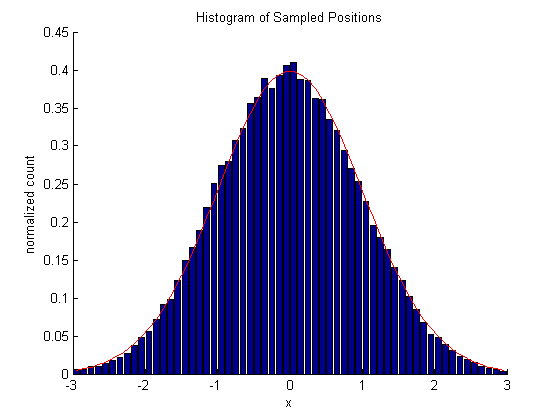
\includegraphics[scale=0.5]{prob2b}
    \end{center}

  \item Below are the plots of our histograms for all of our trials. I decided to use a line plot as opposed to the traditional bar plots for histograms as I thought it would be easier to view. All of the simulations were run for $100,000$ steps.

      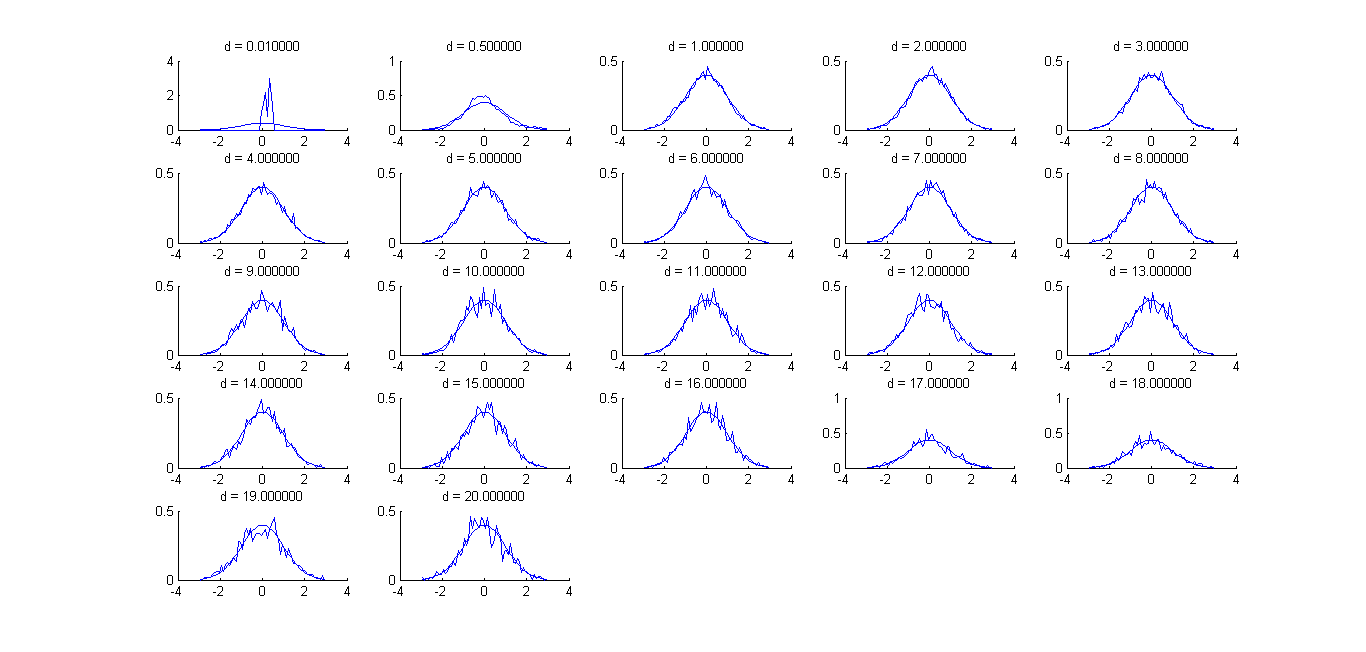
\includegraphics[scale=0.5]{prob2c}

    The table below displays the $f_{acc}$ values for each step $d$\\
    \begin{center}
    $\begin{array}{c|c}
      d & f_{acc} \\ 
      0.01 & 0.9998 \\ 
      0.50 & 0.9582 \\ 
      1.00 & 0.9047 \\ 
      2.00 & 0.8151 \\ 
      3.00 & 0.7127 \\ 
      4.00 & 0.6349 \\ 
      5.00 & 0.5580 \\ 
      6.00 & 0.4975 \\ 
      7.00 & 0.4409 \\ 
      8.00 & 0.3880 \\ 
      9.00 & 0.3455 \\ 
      10.00 & 0.3226 \\ 
      11.00 & 0.2911 \\ 
      12.00 & 0.2607 \\ 
      13.00 & 0.2472 \\ 
      14.00 & 0.2307 \\ 
      15.00 & 0.2065 \\ 
      16.00 & 0.2046 \\ 
      17.00 & 0.1923 \\ 
      18.00 & 0.1748 \\ 
      19.00 & 0.1714 \\ 
      20.00 & 0.1579 \\ 
    \end{array}$
    \end{center}

  \item In part (i) we noted that $f_{acc}$ close to 0 or 1 would result in low efficiency. Extrapolating, we assume that $f_{acc}$ around 0.5 would result in the most efficient sampling for our simulation. From the results in part (iii), we see that ranges of $4 \leq d \leq 8$ appear to offer high sampling efficiency with $f_{acc} \approx 0.5$ and a histogram that qualitatively looks like what we would ideally expect.

  \item The plots below depict the trajectories for a few MC simulations with different step size $d$:
    \begin{center}
      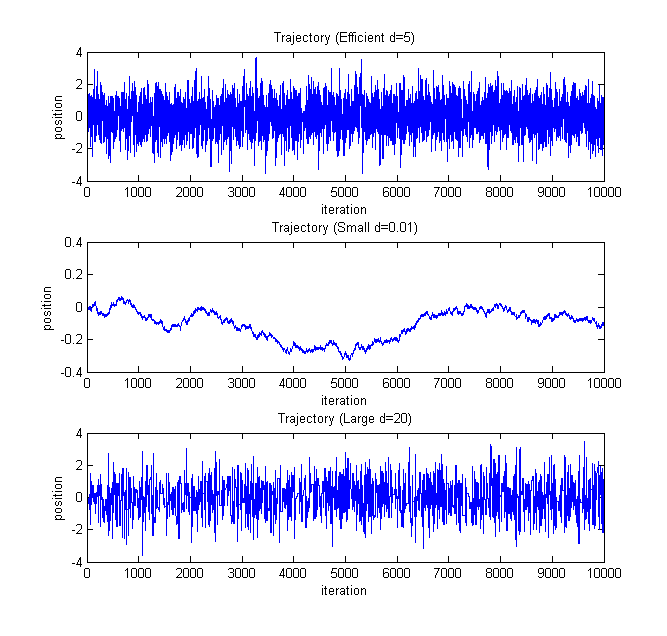
\includegraphics[scale=0.7]{prob2e}
    \end{center}

\end{enumerate}


\section*{Problem 3}
\begin{enumerate}[i.]
  \item Generally, the autocorrelation function for time series results is given by:
    \begin{align}
      C(X(m), X(m+n)) &\propto Cov(X(m), X(m+n)) \\
      &= E\left[ (X(m) - E\left[ X(m) \right]) ((X(m+n) - E\left[ X(m+n) \right])\right]\\
      &= E\left[ X(m) X(m+n)\right] - E\left[X(m)\right] E\left[X(m+n) \right]
    \end{align}

    Since we are sampling from an equilibrium distribution, we can assume translational invariance (on average) with respect to time
    $$E\left[X(m)\right] = E\left[X(m+n)\right] = E\left[X\right]$$
    $$E\left[X(m)X(m+n)\right] = E\left[X((m+i))X((m+i)+n)\right] = E\left[ X(0) X(n)\right]$$

    So we can simplify the correlation function to be solely a function of the separation $n$.
    $$Cov(n) = E\left[ X(0) X(n)\right] - E\left[X\right]^2$$

    In our case $E\left[X \right] = 0$ given that our potential energy function bottoms out at $x=0$. 

  \item Below are our results of $ln|C(n)|$ as a function of $0 \leq n \leq 10$ for various step sizes $d$. Each simulation was run with $100,000$ steps\\
    \begin{center}
      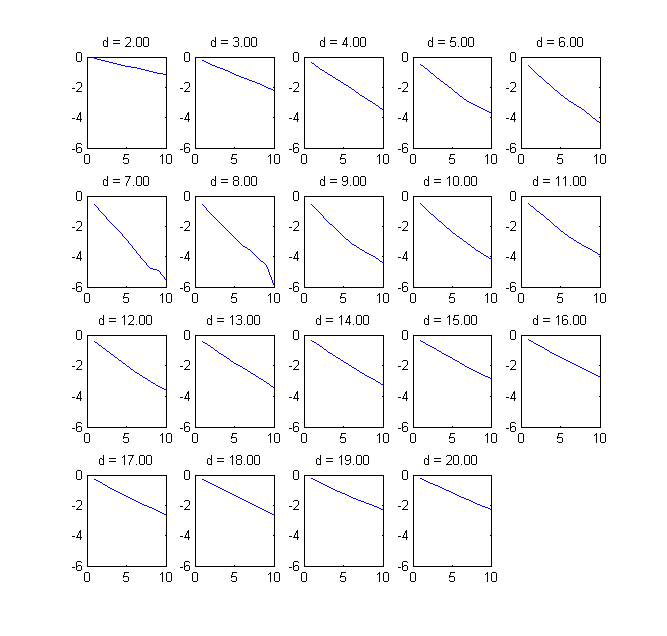
\includegraphics[scale=0.7]{prob3b}
    \end{center}

  \item Using MATLAB's polyfit function with a degree of 1, we fit a line to our results from the previous part. With the slope $k$, we can calculate an estimate for $n_{corr} = 1 / k$. The plots below display our results for $n_{corr}$ as a function of $d$ and $f_{acc}$, respectively
    \begin{center}
      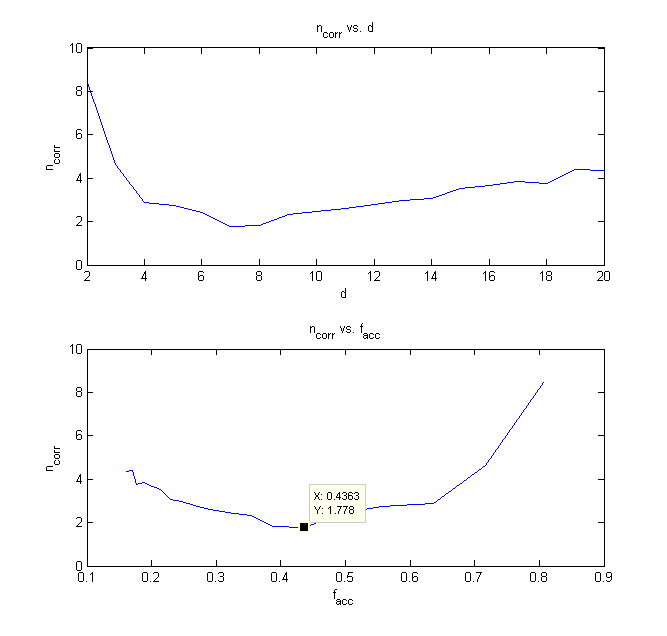
\includegraphics[scale=0.7]{prob3c}
    \end{center}

  \item From part(iii) we see that $0.35 \leq f_{acc} \leq 0.5$, corresponding to $6 \leq d \leq 9$, appears to produce the lowest $n_{corr}$. A lower $n_{corr}$ means a higher efficiency because there are fewer steps on average needed to obtain a statistically independent sample. In problem 2, we assumed that $f_{acc} \approx 0.5$, $d=6$, would make for the most efficient sampling. Now quantitatively, we see that our estimate is slightly off; from part (iii) $f_{acc}=0.4363$, $d=7$, would be most efficient for our simulation with an average $n_{corr}=1.778$.
\end{enumerate}

\section*{Problem 4}
\begin{enumerate}[i.]
  \item At equilibrium, we want to satisfy the ``detailed balance'' condition for the Boltzmann distribution.
    $$\frac{acc(v\rightarrow v')}{acc(v'\rightarrow v)} = \frac{P(v')}{P(v)} = exp\left[-\beta (U(v') - U(v))\right]$$

    From the following we, see that the Glauber criterion does indeed satisfy this condition:
    \begin{align}
      \frac{acc(v\rightarrow v')}{acc(v'\rightarrow v)} &= \frac{exp\left[ -\beta U(v') \right] / exp\left[ -\beta U(v') \right] + exp\left[ -\beta U(v) \right]}{exp\left[ -\beta U(v) \right] / exp\left[ -\beta U(v') \right] + exp\left[ -\beta U(v) \right]} \\
      &= \frac{exp\left[ -\beta U(v') \right]}{exp\left[ -\beta U(v) \right]} \\
      &= exp\left[-\beta (U(v') - U(v))\right]
    \end{align}    

  \item Like in problem 3, plots of $ln|C(n)|$ as functions of $n$ were generated. Each simulation was run for $100,000$ steps.
    \begin{center}
      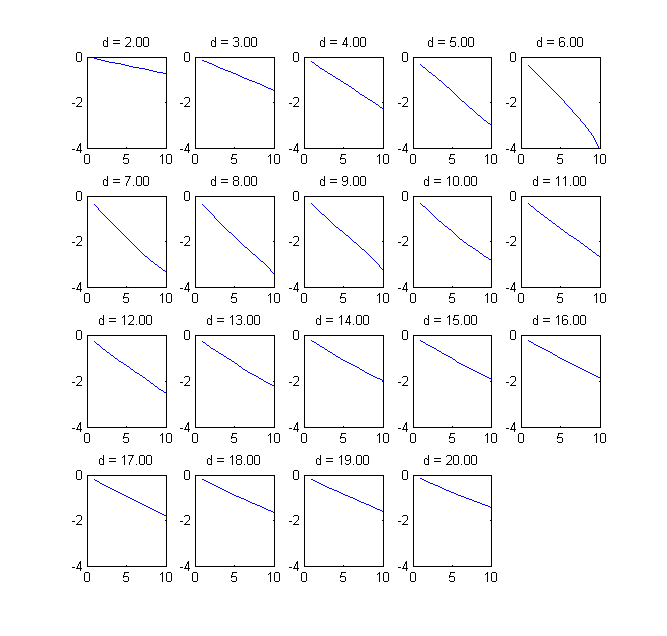
\includegraphics[scale=0.7]{prob4b}
    \end{center}

    From the slopes of the lines above, we found $n_{corr}= 1 / k$ for different values of $d$, with their respective $f_{acc}$. Our results are depicted below:
    \begin{center}
      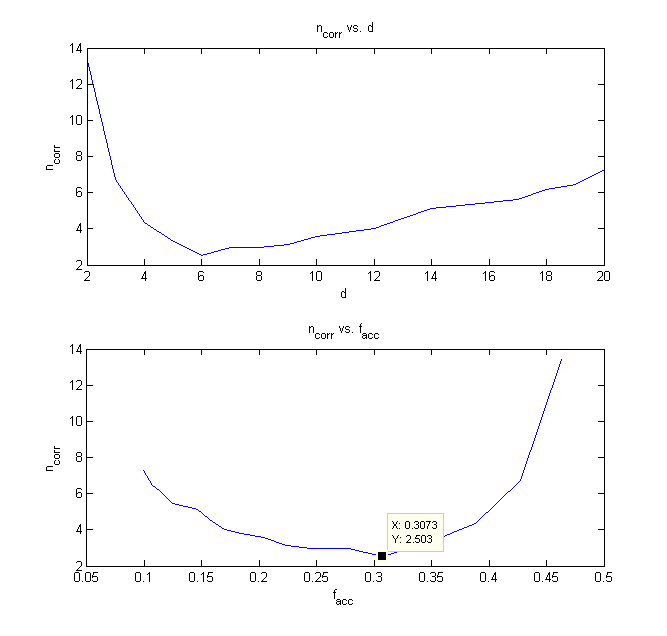
\includegraphics[scale=0.7]{prob4c}
    \end{center}

    From our results we see that the $f_{acc}=0.3073$, $d=6$, provides the besst efficiency with an average $n_{corr}=2.503$.
 
  \item If we measure efficiency based on $n_{corr}$, which is our estimate of the average number of simulation steps to obtain one independent sample, we find that using the Metropolis criterion (min of $n_{corr}= 1.778$ for $d = 7$) is more efficient than the Glauber acceptance rule (min of $n_{corr}=2.503$ for $d = 6$). 
\end{enumerate}

\end{document}
